
\section{Translucent with 1+1 protection}\label{ILP_Transluc_Protection}

\subsection{Model description}

Once more first of all, in order to use the ILP model, we must take into account the physical and logical topologies allowed by this mode of transport and the type of survivability. Through the following figures, you can see these topologies.

\begin{figure}[h!]
\centering
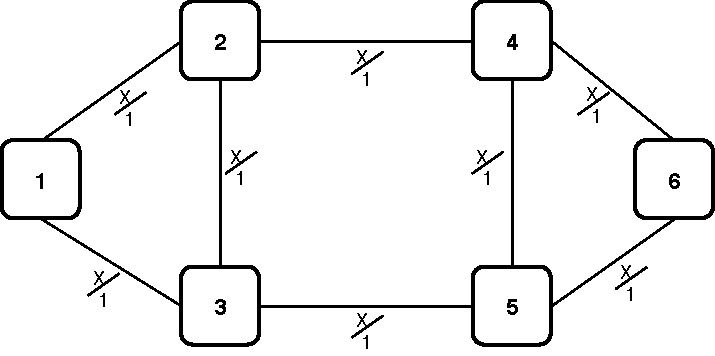
\includegraphics[width=11cm]{sdf/ilp/translucent_protection/figures/allowed_physical_topology}
\caption{Translucent with 1+1 protection: allowed physical topology. The allowed physical topology is defined by the duct and sites in the field. It is assumed that each duct supports up to 1 bidirectional transmission system and each site supports up to 1 node.}
\label{allowed3_physical_protectionlow}
\end{figure}

\newpage
\begin{figure}[h!]
\centering
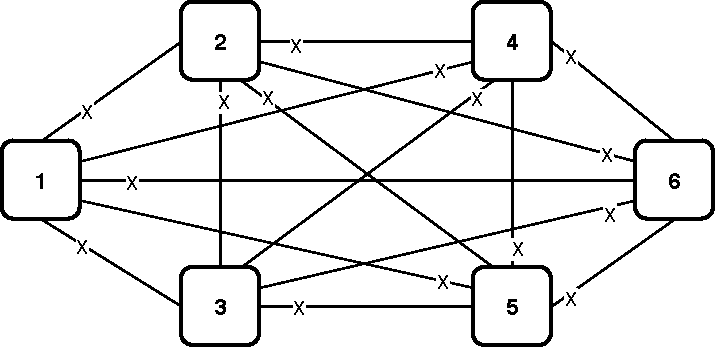
\includegraphics[width=10cm]{sdf/ilp/translucent_protection/figures/allowed_optical_topology}
\caption{Translucent with 1+1 protection: allowed optical topology. The allowed optical topology is defined by the transport mode. It is assumed that each connections between demands supports up to 100 lightpaths.}
\label{allowed3_optical_protectionlow}
\end{figure}

Now taking this into consideration and based on the specific constraints of the translucent mode with 1+1 protection it is possible to define the ILP model \cite{zhu_transl} \cite{zhu_transl2}.\\
The objective function, to be minimized, is the expression \ref{Capex}, i.e.,

\begin{equation*}
  minimize \qquad \Big\{ \quad C_C \quad \Big\}
\end{equation*}

$subject$ $to$
\begin{equation}
\sum_{k=1\textbackslash \{o\}}^{N} Ls_{pk}^{odc} = D_{odc} \qquad \qquad \qquad \qquad \qquad \qquad \qquad
\forall(o,d,c) : o < d, \forall p: p = o
\label{ILPTranslucp1}
\end{equation}
\noindent
Constraint \ref{ILPTranslucp1} is equal to constraint \ref{ILPTransluc1} referred in precedent model.

\begin{equation}
\sum_{k=1\textbackslash \{p,o\}}^{N} Ls_{pk}^{odc} = \sum_{k=1\textbackslash \{p,d\}}^{N} Ls_{kp}^{odc} \qquad \qquad \qquad
\forall(o,d,c) : o < d, \forall p: p \neq o,d
\label{ILPTranslucp2}
\end{equation}
\noindent
Constraint \ref{ILPTranslucp2} is equal to constraint \ref{ILPTransluc2} referred in previous model.

\begin{equation}
\sum_{k=1\textbackslash \{d\}}^{N} Ls_{kp}^{odc} = D_{odc} \qquad \qquad \qquad \qquad \qquad \qquad \qquad \qquad
\forall(o,d,c) : o < d, \forall p: p = d
\label{ILPTranslucp3}
\end{equation}
\noindent
Constraint \ref{ILPTranslucp3} is equal to constraint \ref{ILPTransluc3} referred in precedent model.

\begin{equation}
\sum_{k=1\textbackslash \{o\}}^{N} Lsp_{pk}^{odc} = D_{odc} \qquad \qquad \qquad \qquad \qquad \qquad \qquad
\forall(o,d,c) : o < d, \forall p: p = o
\label{ILPTranslucp1p}
\end{equation}
\noindent
Constraint \ref{ILPTranslucp1p} is the virtual flow conservation constraint and is equal to constraint \ref{ILPTransluc1} but for protection path.

\begin{equation}
\sum_{k=1\textbackslash \{p,o\}}^{N} Lsp_{pk}^{odc} = \sum_{k=1\textbackslash \{p,d\}}^{N} Lsp_{kp}^{odc} \qquad \qquad \qquad
\forall(o,d,c) : o < d, \forall p: p \neq o,d
\label{ILPTranslucp2p}
\end{equation}
\noindent
Constraint \ref{ILPTranslucp2p} is equal to constraint \ref{ILPTransluc2} but for protection path.

\begin{equation}
\sum_{k=1\textbackslash \{d\}}^{N} Lsp_{kp}^{odc} = D_{odc} \qquad \qquad \qquad \qquad \qquad \qquad \qquad
\forall(o,d,c) : o < d, \forall p: p = d
\label{ILPTranslucp3p}
\end{equation}
\noindent
Constraint \ref{ILPTranslucp3p} is equal to constraint \ref{ILPTransluc3} but for virtual protection flow.

\begin{equation}
(Ls_{pk}^{odc} + Lsp_{pk}^{odc}) \leq D_{odc} \qquad \qquad \qquad \qquad \qquad \qquad \qquad \qquad
\forall (p,k), \forall(o,d,c) : o < d
\label{ILPTranslucpX}
\end{equation}
\noindent
The constraint \ref{ILPTranslucpX} assures that the variable $Ls_{pk}^{odc}$ (working flow) and $Lsp_{pk}^{odc}$ (protection flow) are different assigning a different working path than the protection path.

\begin{equation}
\sum_{o=1}^{N} \sum_{d=o+1}^{N} (B(c)(Ls_{pk}^{odc} + Ls_{kp}^{odc} + Lsp_{pk}^{odc} + Lsp_{kp}^{odc})) \leq  \tau \lambda_{pk} \qquad \qquad
\forall (p,k) : p < k, \forall (c)
\label{ILPTranslucp4}
\end{equation}
\noindent
Constraint \ref{ILPTranslucp4} is considered grooming constraint and is equal to constraint \ref{ILPTransluc4}.

\begin{equation}
\sum_{j=1\textbackslash \{p\}}^{N} f_{ij}^{pk} = \lambda_{pk}  \qquad \qquad \qquad \qquad \qquad \qquad \qquad \qquad \qquad
\forall(p,k) : p < k, \forall i: i = p
\label{ILPTranslucp6}
\end{equation}
\noindent
Constraint \ref{ILPTranslucp6} is equal to the constraint \ref{ILPOpaque1_CAPEX} assuming that Z is equal to the number of optical channels between lightpath $(p,k)$.

\begin{equation}
\sum_{j=1\textbackslash \{p\}}^{N} f_{ij}^{pk} = \sum_{j=1\textbackslash \{k\}}^{N} f_{ji}^{pk} \qquad \qquad \qquad \qquad \qquad \qquad
\forall(p,k) : p < k, \forall i: i \neq p,k
\label{ILPTranslucp7}
\end{equation}
\noindent
Constraint \ref{ILPTranslucp7} is equal to the constraint \ref{ILPOpaque2_CAPEX}.

\begin{equation}
\sum_{j=1\textbackslash \{k\}}^{N} f_{ji}^{pk} = \lambda_{pk}  \qquad \qquad \qquad \qquad \qquad \qquad \qquad \qquad \qquad
\forall(p,k) : p < k, \forall i: i = k
\label{ILPTranslucp8}
\end{equation}
\noindent
Constraint \ref{ILPTranslucp8} is equal to the constraint \ref{ILPOpaque3_CAPEX} assuming that Z is equal to the number of optical channels between lightpath $(p,k)$.

\begin{equation}
\sum_{p=1}^{N} \sum_{k=p+1}^{N} \left( f_{ij}^{pk} + f_{ji}^{pk}\right) \leq K_{ij} G_{ij} L_{ij} \qquad \qquad \qquad \qquad \qquad \qquad \qquad
\forall (i,j) : i < j
\label{ILPTranslucp9}
\end{equation}
\noindent
Constraint \ref{ILPTranslucp9} answers the capacity constraint problem and is equal to constraint \ref{ILPTransluc9}.

\begin{equation}
f_{ij}^{pk} , f_{ji}^{pk} , Ls_{pk}^{odc} , Ls_{kp}^{odc} , \lambda_{pk} \in \mathbb{N}   \qquad \qquad \qquad \qquad \qquad
\forall(i,j) : i < j, \forall(o,d) : o < d
\label{ILPTranslucp10}
\end{equation}
\noindent
The constraint \ref{ILPTranslucp10} defines that these variables must be a integer number.

\begin{equation}
L_{i,j} \in \{0,1\} \qquad \qquad \qquad \qquad \qquad \qquad \qquad \qquad \qquad \qquad \qquad \qquad \qquad \qquad
\forall(i,j)
\label{ILPTransluc11}
\end{equation}
\noindent
Last constraint define the variables $L_{ij}$ as binary values.\\

\subsection{Result description}

\textbf{Low Traffic Scenario:}\\

In a first phase, we will show the resulting physical and optical topology based on the allowed topologies and also taking into account the section \ref{low_scenario}.

\begin{figure}[h!]
\centering
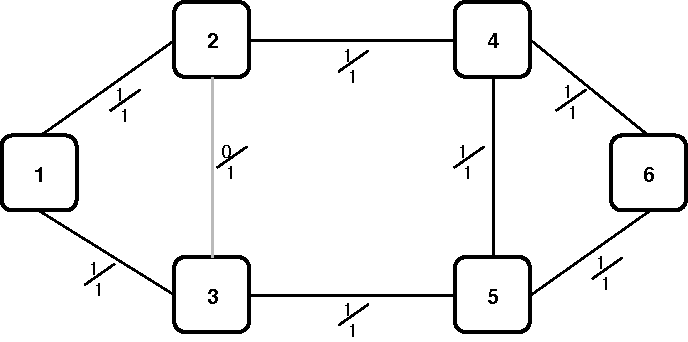
\includegraphics[width=11cm]{sdf/ilp/translucent_protection/figures/physical_topology_low}
\caption{Translucent with 1+1 protection in low scenario: physical topology after dimensioning.}
\label{physical3_protectionlow}
\end{figure}

\newpage
\begin{figure}[h!]
\centering
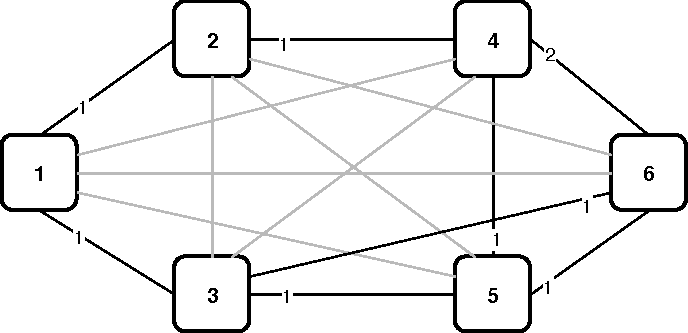
\includegraphics[width=11cm]{sdf/ilp/translucent_protection/figures/optical_topology_low}
\caption{Translucent with 1+1 protection in low scenario: optical topology after dimensioning.}
\label{optical3_protectionlow}
\end{figure}

In table \ref{link_transluc_protec_ref_low} we can see the number of optical channels and the number of amplifiers for each link. In the case where there are no optical channels we assume that the number of amplifiers is zero.

\begin{table}[h!]
\centering
\begin{tabular}{|| c | c | c ||}
 \hline
 \multicolumn{3}{|| c ||}{Information regarding links} \\
 \hline
 \hline
 Bidirectional Link & Optical Channels & Amplifiers\\
 \hline
 Node 1 <-> Node 2 & 1 & 4 \\
 Node 1 <-> Node 3 & 1 & 6 \\
 Node 2 <-> Node 3 & 0 & 0 \\
 Node 2 <-> Node 4 & 1 & 6 \\
 Node 3 <-> Node 5 & 2 & 8 \\
 Node 4 <-> Node 5 & 1 & 1 \\
 Node 4 <-> Node 6 & 2 & 7 \\
 Node 5 <-> Node 6 & 2 & 3 \\
 \hline
\end{tabular}
\caption{Table with information regarding links for translucent mode with 1+1 protection in low scenario.}
\label{link_transluc_protec_ref_low}
\end{table}

In table \ref{node_transluc_protec_ref_low} we can see the resulting nodal degree at the physical layer, the number of line ports and add ports, the number of long-reach transponders and the number of tributary ports.

\begin{table}[h!]
\centering
\begin{tabular}{|| c | c | c | c | c | c ||}
 \hline
 \multicolumn{6}{|| c ||}{Information regarding nodes} \\
 \hline
 \hline
 \multicolumn{2}{|| c |}{ } & \multicolumn{2}{ c |}{Electrical part} & \multicolumn{2}{ c ||}{Optical part} \\
 \hline
 Node & Resulting Nodal Degree & Tributary Ports & LR Transponders & Add Ports & Line Ports\\
 \hline
 1 & 2 & 29 & 2 & 2 & 2 \\
 2 & 2 & 23 & 2 & 2 & 2 \\
 3 & 2 & 18 & 3 & 3 & 3 \\
 4 & 3 & 20 & 4 & 4 & 4 \\
 5 & 3 & 24 & 3 & 3 & 5 \\
 6 & 2 & 22 & 4 & 4 & 4 \\
\hline
\end{tabular}
\caption{Table with information regarding nodes for translucent mode with 1+1 protection in low scenario.}
\label{node_transluc_protec_ref_low}
\end{table}
\newpage
Through the information obtained previously on the nodes we can now create tables with detailed information about each node. In each table mentioned below we can see how many ports are connected to a given node and its bit rate and how many ports are assigned to each different bit rate.\\

\begin{table}[h!]
\centering
\begin{tabular}{|| c | c | c ||}
 \hline
 \multicolumn{3}{|| c ||}{Detailed description of Node 1} \\
 \hline
 \hline
 Electrical part & Number of total demands & Bit rate \\
 \hline
\multirow{3}{*}{29 tributary ports} & 13 & ODU0 \\
 & 13 & ODU1 \\
 & 3 & ODU2 \\
 \hline
  & Node<--Optical Channels-->Node & Bit rate \\
 \hline
 \multirow{2}{*}{2 LR Transponders} & 1  <---- 1 ---->  2 & \multirow{2}{*}{100 Gbits/s} \\
  & 1  <---- 1 ---->  3 & \\
 \hline
 \hline
 Optical part & Node<--Optical Channels-->Node & Bit rate \\
 \hline
 \multirow{2}{*}{2 add ports} & 1  <---- 1 ---->  2 & \multirow{4}{*}{100 Gbits/s} \\
  & 1  <---- 1 ----> 3 & \\ \cline{1-2}
 \multirow{2}{*}{2 line ports} & 1  <---- 1 ---->  2 & \\
  & 1  <---- 1 ----> 3 & \\
\hline
\end{tabular}
\caption{Translucent with 1+1 protection in low scenario: detailed description of node 1. The number of demands is distributed to the various destination nodes, this distribution can be observed in section \ref{low_scenario}.}
\end{table}

\begin{table}[h!]
\centering
\begin{tabular}{|| c | c | c ||}
 \hline
 \multicolumn{3}{|| c ||}{Detailed description of Node 2} \\
 \hline
 \hline
 Electrical part & Number of total demands & Bit rate \\ \hline
\multirow{5}{*}{23 tributary ports} & 11 & ODU0 \\
 & 7 & ODU1 \\
 & 2 & ODU2 \\
 & 2 & ODU3 \\
 & 1 & ODU4 \\
 \hline
  & Node<--Optical Channels-->Node & Bit rate \\
  \hline
\multirow{2}{*}{2 LR Transponders} & 2  <---- 1 ---->  1 & \multirow{2}{*}{100 Gbits/s} \\
  & 2  <---- 1 ---->  4 & \\
 \hline
 \hline
 Optical part & Node<--Optical Channels-->Node & Bit rate \\
 \hline
 \multirow{2}{*}{2 add ports} & 2  <---- 1 ---->  1 & \multirow{4}{*}{100 Gbits/s} \\
  & 2  <---- 1 ---->  4 & \\ \cline{1-2}
 \multirow{2}{*}{2 line ports} & 2  <---- 1 ---->  1 & \\
  & 2  <---- 1 ---->  4 & \\
\hline
\end{tabular}
\caption{Translucent with 1+1 protection in low scenario: detailed description of node 2. The number of demands is distributed to the various destination nodes, this distribution can be observed in section \ref{low_scenario}.}
\end{table}
\newpage
\begin{table}[h!]
\centering
\begin{tabular}{|| c | c | c ||}
 \hline
 \multicolumn{3}{|| c ||}{Detailed description of Node 3} \\
 \hline
 \hline
 Electrical part & Number of total demands & Bit rate \\
 \hline
 \multirow{4}{*}{18 tributary ports} & 7 & ODU0 \\
 & 6 & ODU1\\
 & 3 & ODU2\\
 & 2 & ODU3\\
 \hline
  & Node<--Optical Channels-->Node & Bit rate \\ \hline
 \multirow{3}{*}{3 LR Transponders} & 3  <---- 1 ---->  1 & \multirow{3}{*}{100 Gbits/s} \\
  & 3  <---- 1 ---->  5 & \\
  & 3  <---- 1 ---->  6 & \\
 \hline
 \hline
 Optical part & Node<--Optical Channels-->Node & Bit rate \\
 \hline
 \multirow{3}{*}{3 add ports} & 3  <---- 1 ---->  1 & \multirow{6}{*}{100 Gbits/s} \\
  & 3  <---- 1 ---->  5 & \\
  & 3  <---- 1 ---->  6 & \\  \cline{1-2}
 \multirow{3}{*}{3 line ports} & 3  <---- 1 ---->  1 & \\
  & 3  <---- 1 ---->  5 & \\
  & 3  <---- 1 ---->  6 & \\
\hline
\end{tabular}
\caption{Translucent with 1+1 protection in low scenario: detailed description of node 3. The number of demands is distributed to the various destination nodes, this distribution can be observed in section \ref{low_scenario}.}
\end{table}

\begin{table}[h!]
\centering
\begin{tabular}{|| c | c | c ||}
 \hline
 \multicolumn{3}{|| c ||}{Detailed description of Node 4} \\
 \hline
 \hline
 Electrical part & Number of total demands & Bit rate \\ \hline
\multirow{3}{*}{20 tributary ports} & 7 & ODU0 \\
 & 10 & ODU1 \\
 & 3 & ODU2 \\
 \hline
  & Node<--Optical Channels-->Node & Bit rate \\ \hline
 \multirow{3}{*}{4 LR Transponders} & 4  <---- 1 ---->  2 & \multirow{3}{*}{100 Gbits/s} \\
  & 4  <---- 1 ---->  5 & \\
  & 4  <---- 2 ---->  6 & \\
 \hline
 \hline
 Optical part & Node<--Optical Channels-->Node & Bit rate \\
 \hline
 \multirow{3}{*}{4 add ports} & 4  <---- 1 ---->  2 & \multirow{6}{*}{100 Gbits/s} \\
  & 4  <---- 1 ---->  5 & \\
  & 4  <---- 2 ---->  6 & \\ \cline{1-2}
 \multirow{3}{*}{4 line ports} & 4  <---- 1 ---->  2 & \\
  & 4  <---- 1 ---->  5 & \\
  & 4  <---- 2 ---->  6 & \\
\hline
\end{tabular}
\caption{Translucent with 1+1 protection in low scenario: detailed description of node 4. The number of demands is distributed to the various destination nodes, this distribution can be observed in section \ref{low_scenario}.}
\end{table}
\newpage
\begin{table}[h!]
\centering
\begin{tabular}{|| c | c | c ||}
 \hline
 \multicolumn{3}{|| c ||}{Detailed description of Node 5} \\
 \hline
 \hline
 Electrical part & Number of total demands & Bit rate \\ \hline
\multirow{5}{*}{24 tributary ports} & 14 & ODU0 \\
 & 4 & ODU1 \\
 & 4 & ODU2 \\
 & 1 & ODU3 \\
 & 1 & ODU4 \\
 \hline
  & Node<--Optical Channels-->Node & Bit rate \\ \hline
 \multirow{3}{*}{3 LR Transponders} & 5  <---- 1 ---->  3 & \multirow{3}{*}{100 Gbits/s} \\
  & 5  <---- 1 ---->  4 & \\
  & 5  <---- 1 ---->  6 & \\
 \hline
 \hline
 Optical part & Node<--Optical Channels-->Node & Bit rate \\
 \hline
 \multirow{3}{*}{3 add ports} & 5  <---- 1 ---->  3 & \multirow{7}{*}{100 Gbits/s} \\
  & 5  <---- 1 ---->  4 & \\
  & 5  <---- 1 ---->  6 & \\ \cline{1-2}
 \multirow{4}{*}{5 line ports} & 5  <---- 1 ---->  3 & \\
  & 5  <---- 1 ---->  4 & \\
  & 5  <---- 1 ---->  6 & \\
  & 3  <---- 1 ---->  6 & \\
  \hline
\end{tabular}
\caption{Translucent with 1+1 protection in low scenario: detailed description of node 5. The number of demands is distributed to the various destination nodes, this distribution can be observed in section \ref{low_scenario}.}
\end{table}

\begin{table}[h!]
\centering
\begin{tabular}{|| c | c | c ||}
 \hline
 \multicolumn{3}{|| c ||}{Detailed description of Node 6} \\
 \hline
 \hline
 Electrical part & Number of total demands & Bit rate \\ \hline
\multirow{5}{*}{22 tributary ports} & 8 & ODU0 \\
 & 10 & ODU1 \\
 & 1 & ODU2 \\
 & 1 & ODU3 \\
 & 2 & ODU4 \\
 \hline
  & Node<--Optical Channels-->Node & Bit rate \\ \hline
 \multirow{3}{*}{4 LR Transponders} & 6  <---- 1 ---->  3 & \multirow{3}{*}{100 Gbits/s} \\
  & 6  <---- 2 ---->  4 & \\
  & 6  <---- 1 ---->  5 & \\
 \hline
 Optical part & Node<--Optical Channels-->Node & Bit rate \\
 \hline
 \multirow{3}{*}{4 add ports} & 6  <---- 1 ---->  3 & \multirow{3}{*}{100 Gbits/s} \\
  & 6  <---- 2 ---->  4 & \\
  & 6  <---- 1 ---->  5 & \\ \cline{1-2}
 \multirow{3}{*}{4 line ports} & 6  <---- 1 ---->  3 & \\
  & 6  <---- 2 ---->  4 & \\
  & 6  <---- 1 ---->  5 & \\
\hline
\end{tabular}
\caption{Translucent with 1+1 protection in low scenario: detailed description of node 6. The number of demands is distributed to the various destination nodes, this distribution can be observed in section \ref{low_scenario}.}
\end{table}

\newpage
Now let's focus on the routing information in table \ref{path_transluc_protec_ref_low}. These paths are bidirectional so the path from one node to another is the same path in the opposite direction.\\

\begin{table}[h!]
\centering
\begin{tabular}{||c|c|c|c|c||}
 \hline
 \multicolumn{5}{|| c ||}{Routing} \\
 \hline
 \hline
 o & d & Type & Links & Demands \\
 \hline
 \multirow{2}{*}{1}&\multirow{2}{*}{2}&W&\{(1,3),(3,5),(5,6),(6,4),(4,2)\}&5 ODU0, 2 ODU1, 1 ODU2\\
  & &P& \{(1,2)\} &5 ODU0, 2 ODU1, 1 ODU2 \\ \hline
 \multirow{2}{*}{1}&\multirow{2}{*}{3}&W&\{(1,2),(2,4),(4,6),(6,5),(5,3)\}&1 ODU0, 4 ODU1, 1 ODU2\\
  & &P& \{(1,3)\} & 1 ODU0, 4 ODU1, 1 ODU2 \\ \hline
 \multirow{2}{*}{1} & \multirow{2}{*}{4}&W&\{(1,3),(3,5),(5,6),(6,4)\}&3 ODU0, 2 ODU1, 1 ODU2\\
  & &P& \{(1,2),(2,4)\} & 3 ODU0, 2 ODU1, 1 ODU2 \\ \hline
 \multirow{2}{*}{1} & \multirow{2}{*}{5}&W&\{(1,2),(2,4),(4,5)\}& 1 ODU0\\
  & &P& \{(1,3),(3,5)\} & 1 ODU0 \\ \hline
 \multirow{2}{*}{1} & \multirow{2}{*}{6}&W& \{(1,2),(2,4),(4,6)\} & 3 ODU0, 5 ODU1 \\
  & &P& \{(1,3),(3,5),(5,6)\} & 3 ODU0, 5 ODU1 \\ \hline
 \multirow{2}{*}{2} & \multirow{2}{*}{3}&W& \{(2,4),(4,5),(5,3)\} & 1 ODU3 \\
  & &P& \{(2,1),(1,3)\} & 1 ODU3 \\ \hline
 \multirow{2}{*}{2} & \multirow{2}{*}{4}&W&\{(2,1),(1,3),(3,5),(5,6),(6,4)\}&1 ODU0, 3 ODU1 \\
  & &P& \{(2,4)\} & 1 ODU0, 3 ODU1 \\ \hline
 \multirow{2}{*}{2} & \multirow{2}{*}{5}&W&\{(2,1),(1,3),(3,5)\} & 5 ODU0, 1 ODU1, 1 ODU2 \\
  & &P& \{(2,4),(4,5)\} & 5 ODU0, 1 ODU1, 1 ODU2 \\ \hline
 \multirow{2}{*}{2} & \multirow{2}{*}{6}&W&\{(2,1),(1,3),(3,5),(5,6)\}& 1 ODU1, 1 ODU3, 1 ODU4 \\
  & &P& \{(2,4),(4,6)\} & 1 ODU1, 1 ODU3, 1 ODU4 \\ \hline
 \multirow{2}{*}{3} & \multirow{2}{*}{4}&W& \{(3,1),(1,2),(2,4)\} & 1 ODU0, 1 ODU1, 1 ODU2 \\
  & &P& \{(3,5),(5,6),(6,4)\} & 1 ODU0, 1 ODU1, 1 ODU2 \\ \hline
 \multirow{2}{*}{3}&\multirow{2}{*}{5}&W&\{(3,5),(5,6),(6,4),(4,5)\}&4 ODU0, 1 ODU1, 1 ODU2, 1 ODU3\\
  & &P& \{(3,5)\} & 4 ODU0, 1 ODU1, 1 ODU2, 1 ODU3 \\ \hline
 \multirow{2}{*}{3} & \multirow{2}{*}{6}&W& \{(3,5),(5,6)\} & 1 ODU0 \\
  & &P& \{(3,5),(5,6)\} & 1 ODU0 \\ \hline
 \multirow{2}{*}{4} & \multirow{2}{*}{5}&W& \{(4,6),(6,5),(5,3),(3,5)\} & 1 ODU0, 1 ODU1, 1 ODU2 \\
  & &P& \{(4,5)\} & 1 ODU0, 1 ODU1, 1 ODU2 \\ \hline
 \multirow{2}{*}{4} & \multirow{2}{*}{6}&W& \{(4,5),(5,6)\} & 1 ODU0, 3 ODU1\\
  & &P& \{(4,6)\} & 1 ODU0, 3 ODU1\\ \hline
 \multirow{3}{*}{5} & \multirow{3}{*}{6}&W&\{(5,3),(3,5),(5,6)\}& 3 ODU0, 1 ODU1, 1 ODU2 \\
  & &W& \{(5,4),(4,6)\} & 1 ODU4 \\
  & &P& \{(5,6)\}& 3 ODU0, 1 ODU1, 1 ODU2, 1 ODU4 \\ \hline
\end{tabular}
\caption{Translucent with 1+1 protection in low scenario: description of demands routing. The type W means that it is working path and type P protection path.}
\label{path_transluc_protec_ref_low}
\end{table}

Lastly and most importantly through table \ref{scripttransluc_protec_ref_low} we can see the CAPEX result for this model. This value is obtained using equation \ref{ILPOpaque_CAPEX} and all of the constraints mentioned above.\\
\newpage
\begin{table}[h!]
\centering
\begin{tabular}{||c|c|c|c|c|c|c||}
 \hline
 \multicolumn{7}{||c||}{CAPEX of the Network} \\
 \hline
 \hline
 \multicolumn{3}{||c|}{}&Quantity&Unit Price&Cost&Total \\
 \hline
 \multirow{3}{*}{\makecell{Link \\ Cost}} &\multicolumn{2}{c|}{OLTs}&14&15 000 \euro&210 000 \euro&\multirow{3}{*}{10 490 000 \euro} \\ \cline{2-6}
 &\multicolumn{2}{c|}{100 Gbits/s Transceivers}&20&5 000 \euro/Gbit/s&10 000 000 \euro&\\ \cline{2-6}
 &\multicolumn{2}{c|}{Amplifiers}&70&4 000 \euro&280 000 \euro& \\
 \hline
 \multirow{10}{*}{\makecell{Node \\ Cost}} &\multirow{7}{*}{Electrical}&EXCs&6&10 000 \euro&60 000 \euro&\multirow{10}{*}{2 077 590 \euro}\\ \cline{3-6}
 & &ODU0 Ports&60&10 \euro/port&600 \euro& \\ \cline{3-6}
 & &ODU1 Ports&50&15 \euro/port&750 \euro& \\ \cline{3-6}
 & &ODU2 Ports&16&30 \euro/port&480 \euro& \\ \cline{3-6}
 & &ODU3 Ports&6&60 \euro/port&360 \euro& \\ \cline{3-6}
 & &ODU4 Ports&4&100 \euro/port&400 \euro& \\ \cline{3-6}
 & &Transponders&18&100 000 \euro/port&1 800 000 \euro& \\ \cline{2-6}
 &\multirow{3}{*}{Optical}&OXCs&6&20 000 \euro&120 000 \euro& \\ \cline{3-6}
 & &Line Ports&20&2 500 \euro/port&50 000 \euro& \\ \cline{3-6}
 & &Add Ports&18&2 500 \euro/port&45 000 \euro& \\
 \hline
 \multicolumn{6}{||c|}{Total Network Cost}&12 567 590 \euro \\
\hline
\end{tabular}
\caption{Translucent with 1+1 protection in low scenario: detailed description of CAPEX for this scenario.}
\label{scripttransluc_protec_ref_low}
\end{table}

\textbf{Medium Traffic Scenario:}\\

In a first phase, we will show the resulting physical and optical topology. These topologies are based on the allowed topologies referred to in the model description and also taking into account the logical topology for all ODUs mentioned in the section \ref{medium_traffic_scenario}.\\

\begin{figure}[h!]
\centering
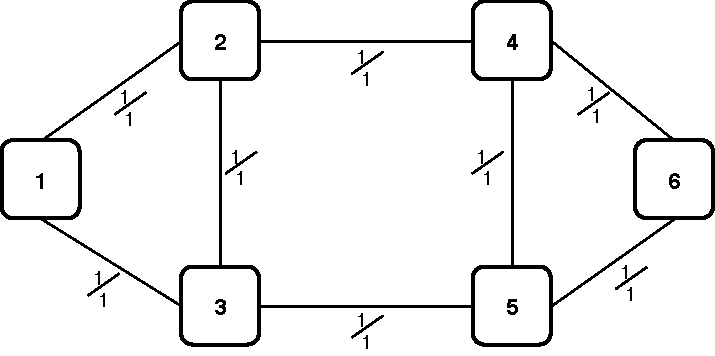
\includegraphics[width=11cm]{sdf/ilp/translucent_protection/figures/physical_topology_medium}
\caption{Translucent with 1+1 protection in medium scenario: physical topology after dimensioning.}
\label{physical3_protectionmedium}
\end{figure}
\newpage
\begin{figure}[h!]
\centering
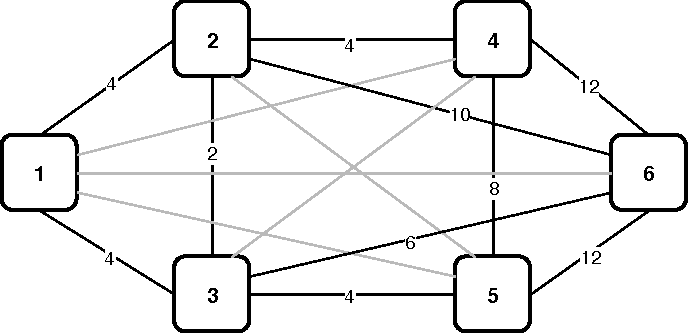
\includegraphics[width=11cm]{sdf/ilp/translucent_protection/figures/optical_topology_medium}
\caption{Translucent with 1+1 protection in medium scenario: optical topology after dimensioning.}
\label{optical3_protectionmedium}
\end{figure}

In table \ref{link_transluc_protec_ref_medium} we can see the number of optical channels calculated using \ref{Capex_Link} and \ref{ILPOpaque_CAPEX} and the number of amplifiers for each link calculated using \ref{Capex_amplifiers}.

\begin{table}[h!]
\centering
\begin{tabular}{|| c | c | c ||}
 \hline
 \multicolumn{3}{|| c ||}{Information regarding links} \\
 \hline
 \hline
 Bidirectional Link & Optical Channels & Amplifiers\\
 \hline
 Node 1 <-> Node 2 & 4 & 4 \\
 Node 1 <-> Node 3 & 4 & 6 \\
 Node 2 <-> Node 3 & 2 & 0 \\
 Node 2 <-> Node 4 & 14 & 6 \\
 Node 3 <-> Node 5 & 10 & 8 \\
 Node 4 <-> Node 5 & 8 & 1 \\
 Node 4 <-> Node 6 & 22 & 7 \\
 Node 5 <-> Node 6 & 18 & 3 \\
 \hline
\end{tabular}
\caption{Table with information regarding links for translucent mode with 1+1 protection in medium scenario.}
\label{link_transluc_protec_ref_medium}
\end{table}

In table \ref{node_transluc_protec_ref_medium} we can see the resulting nodal degree at the physical layer, the number of line ports and add ports using \ref{OXC_poxc_transluc} the number of long-reach transponders using \ref{EXC_pexc2_transluc} and the number of tributary ports using \ref{EXC_pexc1_transluc}.

\begin{table}[h!]
\centering
\begin{tabular}{|| c | c | c | c | c | c ||}
 \hline
 \multicolumn{6}{|| c ||}{Information regarding nodes} \\
 \hline
 \hline
 \multicolumn{2}{|| c |}{ } & \multicolumn{2}{ c |}{Electrical part} & \multicolumn{2}{ c ||}{Optical part} \\
 \hline
 Node & Resulting Nodal Degree & Tributary Ports & LR Transponders & Add Ports & Line Ports\\
 \hline
 1 & 2 & 290 & 8 & 8 & 8 \\
 2 & 3 & 230 & 20 & 20 & 20 \\
 3 & 3 & 180 & 16 & 16 & 16 \\
 4 & 3 & 200 & 24 & 24 & 44 \\
 5 & 3 & 240 & 24 & 24 & 36 \\
 6 & 2 & 220 & 40 & 40 & 40 \\
\hline
\end{tabular}
\caption{Table with information regarding nodes for translucent mode with 1+1 protection in medium scenario.}
\label{node_transluc_protec_ref_medium}
\end{table}

\newpage
Through the information obtained previously on the nodes we can now create tables with detailed information about each node.

\begin{table}[h!]
\centering
\begin{tabular}{|| c | c | c ||}
 \hline
 \multicolumn{3}{|| c ||}{Detailed description of Node 1} \\
 \hline
 \hline
 Electrical part & Number of total demands & Bit rate \\
 \hline
\multirow{3}{*}{290 tributary ports} & 130 & ODU0 \\
 & 130 & ODU1 \\
 & 30 & ODU2 \\
 \hline
  & Node<--Optical Channels-->Node & Bit rate \\
 \hline
\multirow{2}{*}{8 LR Transponders} & 1  <---- 4 ---->  2 & \multirow{2}{*}{100 Gbits/s} \\
  & 1  <---- 4 ---->  3 & \\
 \hline
 \hline
 Optical part & Node<--Optical Channels-->Node & Bit rate \\
 \hline
 \multirow{2}{*}{8 add ports} & 1  <---- 4 ---->  2 & \multirow{4}{*}{100 Gbits/s} \\
  & 1  <---- 4 ---->  3 & \\ \cline{1-2}
 \multirow{2}{*}{8 line ports} & 1  <---- 4 ---->  2 & \\
  & 1  <---- 4 ---->  3 & \\
\hline
\end{tabular}
\caption{Translucent with 1+1 protection in medium scenario: detailed description of node 1. The number of demands is distributed to the various destination nodes, this distribution can be observed in section \ref{medium_traffic_scenario}.}
\end{table}

\begin{table}[h!]
\centering
\begin{tabular}{|| c | c | c ||}
 \hline
 \multicolumn{3}{|| c ||}{Detailed description of Node 2} \\
 \hline
 \hline
 Electrical part & Number of total demands & Bit rate \\ \hline
\multirow{5}{*}{230 tributary ports} & 110 & ODU0 \\
 & 70 & ODU1 \\
 & 20 & ODU2 \\
 & 20 & ODU3 \\
 & 10 & ODU4 \\
 \hline
  & Node<--Optical Channels-->Node & Bit rate \\
  \hline
\multirow{4}{*}{20 LR Transponders} & 2  <---- 4 ---->  1 & \multirow{4}{*}{100 Gbits/s} \\
  & 2  <---- 2 ---->  3 & \\
  & 2  <---- 4 ---->  4 & \\
  & 2  <---- 10 ---->  6 & \\
 \hline
 \hline
 Optical part & Node<--Optical Channels-->Node & Bit rate \\
 \hline
 \multirow{4}{*}{20 add ports} & 2  <---- 4 ---->  1 & \multirow{8}{*}{100 Gbits/s} \\
  & 2  <---- 2 ---->  3 & \\
  & 2  <---- 4 ---->  4 & \\
  & 2  <---- 10 ---->  6 & \\ \cline{1-2}
 \multirow{4}{*}{20 line ports} & 2  <---- 4 ---->  1 & \\
  & 2  <---- 2 ---->  3 & \\
  & 2  <---- 4 ---->  4 & \\
  & 2  <---- 10 ---->  6 & \\
\hline
\end{tabular}
\caption{Translucent with 1+1 protection in medium scenario: detailed description of node 2. The number of demands is distributed to the various destination nodes, this distribution can be observed in section \ref{medium_traffic_scenario}.}
\end{table}

\newpage
\begin{table}[h!]
\centering
\begin{tabular}{|| c | c | c ||}
 \hline
 \multicolumn{3}{|| c ||}{Detailed description of Node 3} \\
 \hline
 \hline
 Electrical part & Number of total demands & Bit rate \\
 \hline
 \multirow{4}{*}{180 tributary ports} & 70 & ODU0 \\
 & 60 & ODU1\\
 & 30 & ODU2\\
 & 20 & ODU3\\
 \hline
  & Node<--Optical Channels-->Node & Bit rate \\ \hline
 \multirow{4}{*}{16 LR Transponders} & 3  <---- 4 ---->  1 & \multirow{4}{*}{100 Gbits/s} \\
  & 3  <---- 2 ---->  2 & \\
  & 3  <---- 4 ---->  5 & \\
  & 3  <---- 6 ---->  6 & \\
 \hline
 \hline
 Optical part & Node<--Optical Channels-->Node & Bit rate \\
 \hline
 \multirow{4}{*}{16 add ports} & 3  <---- 4 ---->  1 & \multirow{8}{*}{100 Gbits/s} \\
  & 3  <---- 2 ---->  2 & \\
  & 3  <---- 4 ---->  5 & \\
  & 3  <---- 6 ---->  6 & \\ \cline{1-2}
 \multirow{4}{*}{16 line ports} & 3  <---- 4 ---->  1 & \\
  & 3  <---- 2 ---->  2 & \\
  & 3  <---- 4 ---->  5 & \\
  & 3  <---- 6 ---->  6 & \\
\hline
\end{tabular}
\caption{Translucent with 1+1 protection in medium scenario: detailed description of node 3. The number of demands is distributed to the various destination nodes, this distribution can be observed in section \ref{medium_traffic_scenario}.}
\end{table}

\begin{table}[h!]
\centering
\begin{tabular}{|| c | c | c ||}
 \hline
 \multicolumn{3}{|| c ||}{Detailed description of Node 4} \\
 \hline
 \hline
 Electrical part & Number of total demands & Bit rate \\ \hline
\multirow{3}{*}{200 tributary ports} & 70 & ODU0 \\
 & 100 & ODU1 \\
 & 30 & ODU2 \\
 \hline
  & Node<--Optical Channels-->Node & Bit rate \\ \hline
 \multirow{3}{*}{24 LR Transponders} & 4  <---- 4 ---->  2 & \multirow{3}{*}{100 Gbits/s} \\
  & 4  <---- 8 ---->  5 & \\
  & 4  <---- 12 ---->  6 & \\
 \hline
 \hline
 Optical part & Node<--Optical Channels-->Node & Bit rate \\
 \hline
 \multirow{3}{*}{24 add ports} & 4  <---- 4 ---->  2 & \multirow{7}{*}{100 Gbits/s} \\
  & 4  <---- 8 ---->  5 & \\
  & 4  <---- 12 ---->  6 & \\ \cline{1-2}
 \multirow{4}{*}{44 line ports} & 4  <---- 4 ---->  2 & \\
  & 4  <---- 8 ---->  5 & \\
  & 4  <---- 12 ---->  6 & \\
  & 2  <---- 10 ---->  6 & \\
\hline
\end{tabular}
\caption{Translucent with 1+1 protection in medium scenario: detailed description of node 4. The number of demands is distributed to the various destination nodes, this distribution can be observed in section \ref{medium_traffic_scenario}.}
\end{table}

\newpage
\begin{table}[h!]
\centering
\begin{tabular}{|| c | c | c ||}
 \hline
 \multicolumn{3}{|| c ||}{Detailed description of Node 5} \\
 \hline
 \hline
 Electrical part & Number of total demands & Bit rate \\ \hline
\multirow{5}{*}{240 tributary ports} & 140 & ODU0 \\
 & 40 & ODU1 \\
 & 40 & ODU2 \\
 & 10 & ODU3 \\
 & 10 & ODU4 \\
 \hline
  & Node<--Optical Channels-->Node & Bit rate \\ \hline
 \multirow{3}{*}{24 LR Transponders} & 5  <---- 4 ---->  3 & \multirow{3}{*}{100 Gbits/s} \\
  & 5  <---- 8 ---->  4 & \\
  & 5  <---- 12 ---->  6 & \\
 \hline
 \hline
 Optical part & Node<--Optical Channels-->Node & Bit rate \\
 \hline
 \multirow{3}{*}{24 add ports} & 5  <---- 4 ---->  3 & \multirow{7}{*}{100 Gbits/s} \\
  & 5  <---- 8 ---->  4 & \\
  & 5  <---- 12 ---->  6 & \\ \cline{1-2}
 \multirow{4}{*}{36 line ports} & 5  <---- 4 ---->  3 & \\
  & 5  <---- 8 ---->  4 & \\
  & 5  <---- 12 ---->  6 & \\
  & 3  <---- 6 ---->  6 & \\
\hline
\end{tabular}
\caption{Translucent with 1+1 protection in medium scenario: detailed description of node 5. The number of demands is distributed to the various destination nodes can be observed in section \ref{medium_traffic_scenario}.}
\end{table}

\begin{table}[h!]
\centering
\begin{tabular}{|| c | c | c ||}
 \hline
 \multicolumn{3}{|| c ||}{Detailed description of Node 6} \\
 \hline
 \hline
 Electrical part & Number of total demands & Bit rate \\ \hline
\multirow{5}{*}{220 tributary ports} & 80 & ODU0 \\
 & 100 & ODU1 \\
 & 10 & ODU2 \\
 & 10 & ODU3 \\
 & 20 & ODU4 \\
 \hline
  & Node<--Optical Channels-->Node & Bit rate \\ \hline
 \multirow{4}{*}{40 LR Transponders} & 6  <---- 10 ---->  2 & \multirow{4}{*}{100 Gbits/s} \\
  & 6  <---- 6 ---->  3 & \\
  & 6  <---- 12 ---->  4 & \\
  & 6  <---- 12 ---->  5 & \\
 \hline
 Optical part & Node<--Optical Channels-->Node & Bit rate \\
 \hline
 \multirow{4}{*}{40 add ports} & 6  <---- 10 ---->  2 & \multirow{8}{*}{100 Gbits/s} \\
  & 6  <---- 6 ---->  3 & \\
  & 6  <---- 12 ---->  4 & \\
  & 6  <---- 12 ---->  5 & \\ \cline{1-2}
 \multirow{4}{*}{40 line ports} & 6  <---- 10 ---->  2 & \\
  & 6  <---- 6 ---->  3 & \\
  & 6  <---- 12 ---->  4 & \\
  & 6  <---- 12 ---->  5 & \\
\hline
\end{tabular}
\caption{Translucent with 1+1 protection in medium scenario: detailed description of node 6. The number of demands is distributed to the various destination nodes, can be observed in section \ref{medium_traffic_scenario}.}
\end{table}

\newpage
Now through table \ref{scripttransluc_protec_ref_medium} we can see the CAPEX result for this model. This value is obtained using equation \ref{Capex} and all of the constraints mentioned above. \\

\begin{table}[h!]
\centering
\begin{tabular}{||c|c|c|c|c|c|c||}
 \hline
 \multicolumn{7}{||c||}{CAPEX of the Network} \\
 \hline
 \hline
 \multicolumn{3}{||c|}{}&Quantity&Unit Price&Cost&Total \\
 \hline
 \multirow{3}{*}{\makecell{Link \\ Cost}}&\multicolumn{2}{c|}{OLTs}&16&15 000 \euro&240 000 \euro&\multirow{3}{*}{82 520 000 \euro} \\ \cline{2-6}
 &\multicolumn{2}{c|}{100 Gbits/s Transceivers}&164&5 000 \euro/Gbit/s&82 000 000 \euro& \\ \cline{2-6}
 &\multicolumn{2}{c|}{Amplifiers}&70&4 000 \euro&280 000 \euro& \\
 \hline
 \multirow{10}{*}{\makecell{Node \\ Cost}}&\multirow{7}{*}{Electrical}&EXCs&6&10 000 \euro&60 000 \euro&\multirow{10}{*}{14 145 900 \euro} \\ \cline{3-6}
 & &ODU0 Ports&600&10 \euro/port&6 000 \euro& \\ \cline{3-6}
 & &ODU1 Ports&500&15 \euro/port&7 500 \euro& \\ \cline{3-6}
 & &ODU2 Ports&160&30 \euro/port&4 800 \euro& \\ \cline{3-6}
 & &ODU3 Ports&60&60 \euro/port&3 600 \euro& \\ \cline{3-6}
 & &ODU4 Ports&40&100 \euro/port&4 000 \euro& \\ \cline{3-6}
 & &Transponders&132&100 000 \euro/port&13 200 000 \euro& \\ \cline{2-6}
 &\multirow{3}{*}{Optical}&OXCs&6&20 000 \euro&120 000 \euro& \\ \cline{3-6}
 & &Line Ports&164&2 500 \euro/port&410 000 \euro& \\ \cline{3-6}
 & &Add Ports&132&2 500 \euro/port&330 000 \euro& \\
 \hline
 \multicolumn{6}{||c|}{Total Network Cost}&96 665 900 \euro \\
\hline
\end{tabular}
\caption{Translucent with 1+1 protection in medium scenario: detailed description of CAPEX for this scenario.}
\label{scripttransluc_protec_ref_medium}
\end{table}

\vspace{17pt}
In next page, we can see the routing information. These paths are bidirectional so the path from one node to another is the same path in the opposite direction.\\
\newpage
\begin{table}[h]
\centering
\begin{tabular}{||c|c|c|c|c||}
 \hline
 \multicolumn{5}{|| c ||}{Routing} \\
 \hline
 \hline
 o & d & Type & Links & Demands \\
 \hline
 \multirow{2}{*}{1}&\multirow{2}{*}{2}&W&\{(1,3),(3,5),(5,6),(6,4),(4,2)\}&50 ODU0, 20 ODU1, 10 ODU2\\
  & &P& \{(1,2)\} &50 ODU0, 20 ODU1, 10 ODU2 \\ \hline
 \multirow{2}{*}{1}&\multirow{2}{*}{3}&W& \{(1,2),(2,3)\} & 10 ODU0, 40 ODU1, 10 ODU2\\
  & &P& \{(1,3)\} & 10 ODU0, 40 ODU1, 10 ODU2 \\ \hline
 \multirow{2}{*}{1} & \multirow{2}{*}{4}&W&\{(1,3),(3,5),(5,6),(6,4)\}&30 ODU0, 20 ODU1, 10 ODU2\\
  & &P& \{(1,2),(2,4)\} & 30 ODU0, 20 ODU1, 10 ODU2 \\ \hline
 \multirow{2}{*}{1} & \multirow{2}{*}{5}&W&\{(1,2),(2,4),(4,5)\}& 10 ODU0\\
  & &P& \{(1,3),(3,5)\} & 10 ODU0 \\ \hline
 \multirow{2}{*}{1} & \multirow{2}{*}{6}&W& \{(1,3),(3,5),(5,6)\} & 30 ODU0, 50 ODU1 \\
  & &P& \{(1,2),(2,4),(4,6)\} & 30 ODU0, 50 ODU1 \\ \hline
 \multirow{4}{*}{2} & \multirow{4}{*}{3}&W& \{(2,1),(1,3)\} & 5 ODU3 \\
  & &W& \{(2,4),(4,6),(6,5),(5,3)\} & 5 ODU3 \\
  & &P& \{(2,3)\} & 5 ODU3 \\
  & &P& \{(2,1),(1,3)\} & 5 ODU3 \\ \hline
 \multirow{2}{*}{2} & \multirow{2}{*}{4}&W&\{(2,4),(4,6),(6,4)\}&10 ODU0, 30 ODU1 \\
  & &P& \{(2,4)\} & 10 ODU0, 30 ODU1 \\ \hline
 \multirow{4}{*}{2} & \multirow{4}{*}{5}&W&\{(2,4),(4,5)\} & 50 ODU0, 10 ODU1 \\
  & &W& \{(2,1),(1,3),(3,5)\} & 10 ODU2 \\
  & &P& \{(2,3),(3,5)\} & 50 ODU0, 10 ODU1 \\
  & &P& \{(2,4),(4,5)\} & 10 ODU2 \\ \hline
 \multirow{4}{*}{2} & \multirow{4}{*}{6}&W&\{(2,3),(3,5),(5,6)\}& 10 ODU1, 2 ODU4 \\
  & &W& \{(2,4),(4,6)\} & 10 0DU3, 4 ODU4 \\
  & &W& \{(2,1),(1,3),(3,5),(5,6)\} & 4 ODU4 \\
  & &P& \{(2,4),(4,6)\} & 10 ODU1, 10 ODU3, 10 ODU4 \\ \hline
 \multirow{2}{*}{3} & \multirow{2}{*}{4}&W& \{(3,5),(5,6),(6,4)\} & 10 ODU0, 10 ODU1, 10 ODU2 \\
  & &P& \{(3,2),(2,4)\} & 10 ODU0, 10 ODU1, 10 ODU2 \\ \hline
 \multirow{3}{*}{3}&\multirow{3}{*}{5}&W&\{(3,2),(2,4),(4,5)\}&40 ODU0, 10 ODU1 \\
  & &W& \{(3,5),(5,6),(6,4),(4,5)\}& 10 ODU2, 10 ODU3\\
  & &P& \{(3,5)\} & 40 ODU0, 10 ODU1, 10 ODU2, 10 ODU3 \\ \hline
 \multirow{2}{*}{3} & \multirow{2}{*}{6}&W& \{(3,2),(2,4),(4,6)\} & 10 ODU0 \\
  & &P& \{(3,6)\} & 10 ODU0 \\ \hline
 \multirow{3}{*}{4} & \multirow{3}{*}{5}&W& \{(4,2),(2,3),(3,5)\} & 10 ODU0 \\
  & &W& \{(4,6),(6,5),(5,3),(3,5)\} & 10 ODU1, 10 ODU2 \\
  & &P& \{(4,5)\} & 10 ODU0, 10 ODU1, 10 ODU2 \\ \hline
 \multirow{2}{*}{4} & \multirow{2}{*}{6}&W& \{(4,2),(2,4),(4,6)\} & 10 ODU0, 30 ODU1\\
  & &P& \{(4,6)\} & 10 ODU0, 30 ODU1\\ \hline
 \multirow{3}{*}{5} & \multirow{3}{*}{6}&W&\{(5,3),(3,5),(5,6)\}& 30 ODU0, 10 ODU1, 10 ODU2, 2 ODU4 \\
  & &W& \{(5,4),(4,6)\} & 8 ODU4 \\
  & &P& \{(5,6)\}& 30 ODU0, 10 ODU1, 10 ODU2, 10 ODU4 \\ \hline
\end{tabular}
\caption{Translucent with 1+1 protection in medium scenario: description of demands routing. The type W means that it is working path and type P protection path.}
\label{path_transluc_protec_ref_medium}
\end{table}
\newpage
